% Skip over this boring header down a bit
%%%%%%%%%%%%%%%%%%%%%%%%%%%%%%%%%%%%%%%%%%%%%%%%
\documentclass[usenames,dvipsnames,10pt,aspectratio=169]{beamer} 
% Add option 'aspectratio=169' for 16:9 widescreen 
% Add option  'handout' to ignore animations
% If you have a smaller amount of text, feel free to also try '11pt'! / Jesper

\usepackage[utf8]{inputenc}
\usepackage{verbatim}
\usepackage{minted}
\usemintedstyle{monokai}
\usepackage{graphicx}
\usepackage{wrapfig}
\usepackage[document]{ragged2e}
\usetheme{umu}

\usepackage{hyperref}
\hypersetup{
    colorlinks=true,
    linkcolor=ucuyellow,
    filecolor=ucuyellow,      
    urlcolor=ucuyellow,
}
\urlstyle{same}

\usepackage[shortlabels]{enumitem}

%%% Bibliography
\usepackage[style=authoryear,backend=biber]{biblatex}
\addbibresource{bibliography.bib}

\DeclareNameAlias{author}{given-family}

%%% Suppress biblatex annoying warning
\usepackage{silence}
\WarningFilter{biblatex}{Patching footnotes failed}

%%% Some useful commands
% pdf-friendly newline in links
\newcommand{\pdfnewline}{\texorpdfstring{\newline}{ }} 
% Fill the vertical space in a slide (to put text at the bottom)
\newcommand{\framefill}{\vskip0pt plus 1filll}

%%% Enter additional packages below 
\renewcommand{\proofname}{\sffamily{Proof}}

%%%%%%%%%%%%%%%%%%%%%%%%%%%%%%%%%%%%%%%%%%%%%%%%%%%%%%%%%%%%%%%%%%%%%%%%%%%%%%%%%%%%%
\title[Rust \#1]{Rust \#1: Motivation \\ \vspace{0.1cm}and Introduction}
\author[Sultanov Andriy]{Sultanov Andriy}
\institute{APPS@UCU}

\begin{document}

\begin{frame}
\titlepage
\end{frame}

\begin{frame}{\contentsname}
\tableofcontents
\end{frame}

\framepic{graphics/1.jpg}{
 \textcolor{ucuwhite}{What are we doing here?}
 \vskip 0.5cm
 }

\section{What are we doing here?}

\begin{frame}{Why are we here?}
\Large	
We are here to learn a new way \\
of thinking about complex computer \\
systems with the help of the Rust \\
programming language.\\
\end{frame}

\begin{frame}{What this entails}
\large	
We will have to do a few things in order to gain\\
the most in the short amount of time we have:\\
\vspace{0.4cm}
\begin{itemize}[label=$\bullet$]
	\item Listen and ask questions during the lecture
	\item Complete short homework exercises
	\item Work our way through a final group project
	\item Read/Watch/Listen/Do anything and everything\\ 
		we can lay our eyes upon!
\end{itemize}
\end{frame}

\begin{frame}{Rust doesn't solve all of your problems}
\large
While Rust does solve most memory safety issues\\
(more on this later), most bugs are still caused\\
by tired and underslept programmers.\\
\vspace{0.2cm}
\textcolor{ucuyellow}{Your health is more important than your work.}\\
\end{frame}

\begin{frame}{Rust doesn't solve all of your problems}
\large
\textcolor{ucuyellow}{
Developing more secure and memory-safe code in\\
abstract sounds good. But it's not always.\\
}
\vspace{0.4cm}

Developing a secure drone strike system won't help anyone.\\
\vspace{0.2cm}

Secure face recognition system for the police won't help anyone either.\\
\vspace{0.2cm}

A secure app that serves as a tool to further underpay and\\
undermine the vulnerable workforce will bring far more trouble\\
if it's unhackable using simple memory exploits.
\end{frame}


\framepic{graphics/1.jpg}{
\textcolor{ucuwhite}{Motivation}
 \vskip 0.5cm
 }
 
\section{Motivation}%
 
\begin{frame}{Who is interested in Rust?}
	%Leaving all the technical points for later	
	\large
	\textcolor{ucuyellow}{Rust is the most loved language for the fifth year in a row!}\\
	\footnotesize{(86.\% of StackOverflow users)}

	\vspace{0.5cm}

	\large
	Rust is used in production in an increasing number\\
	of companies: Mozilla, Atlassian, Microsoft, Google,\\
	Godot, 1Password, Dropbox, Zeplin, npm, Academia.edu,\\
	Sentry, Cloudflare, Coursera, Figma, Postmates etc.

	\vspace{0.5cm}

	\large
	But Rust's concepts will help in many\\
	other languages as well!
\end{frame} 

\begin{frame}{Why should you be interested in Rust?}
	\large
	Rust is an extremely interesting and relatively\\
	new language that can be used in a lot of\\
	domains, including, but not limited to:\\
	\vspace{0.4cm}
	\begin{itemize}[label=$\bullet$]
		\item Web through WebAssembly
		\item Operating Systems
		\item Embedded Software
		\item Large Systems Software\\
			(Browsers, Servers, Databases etc.)
		\item Games, GUI, CLI applications too!
	\end{itemize}
\end{frame}

\begin{frame}{Resources}
	\Large
	\centering
	\begin{figure}[c]
		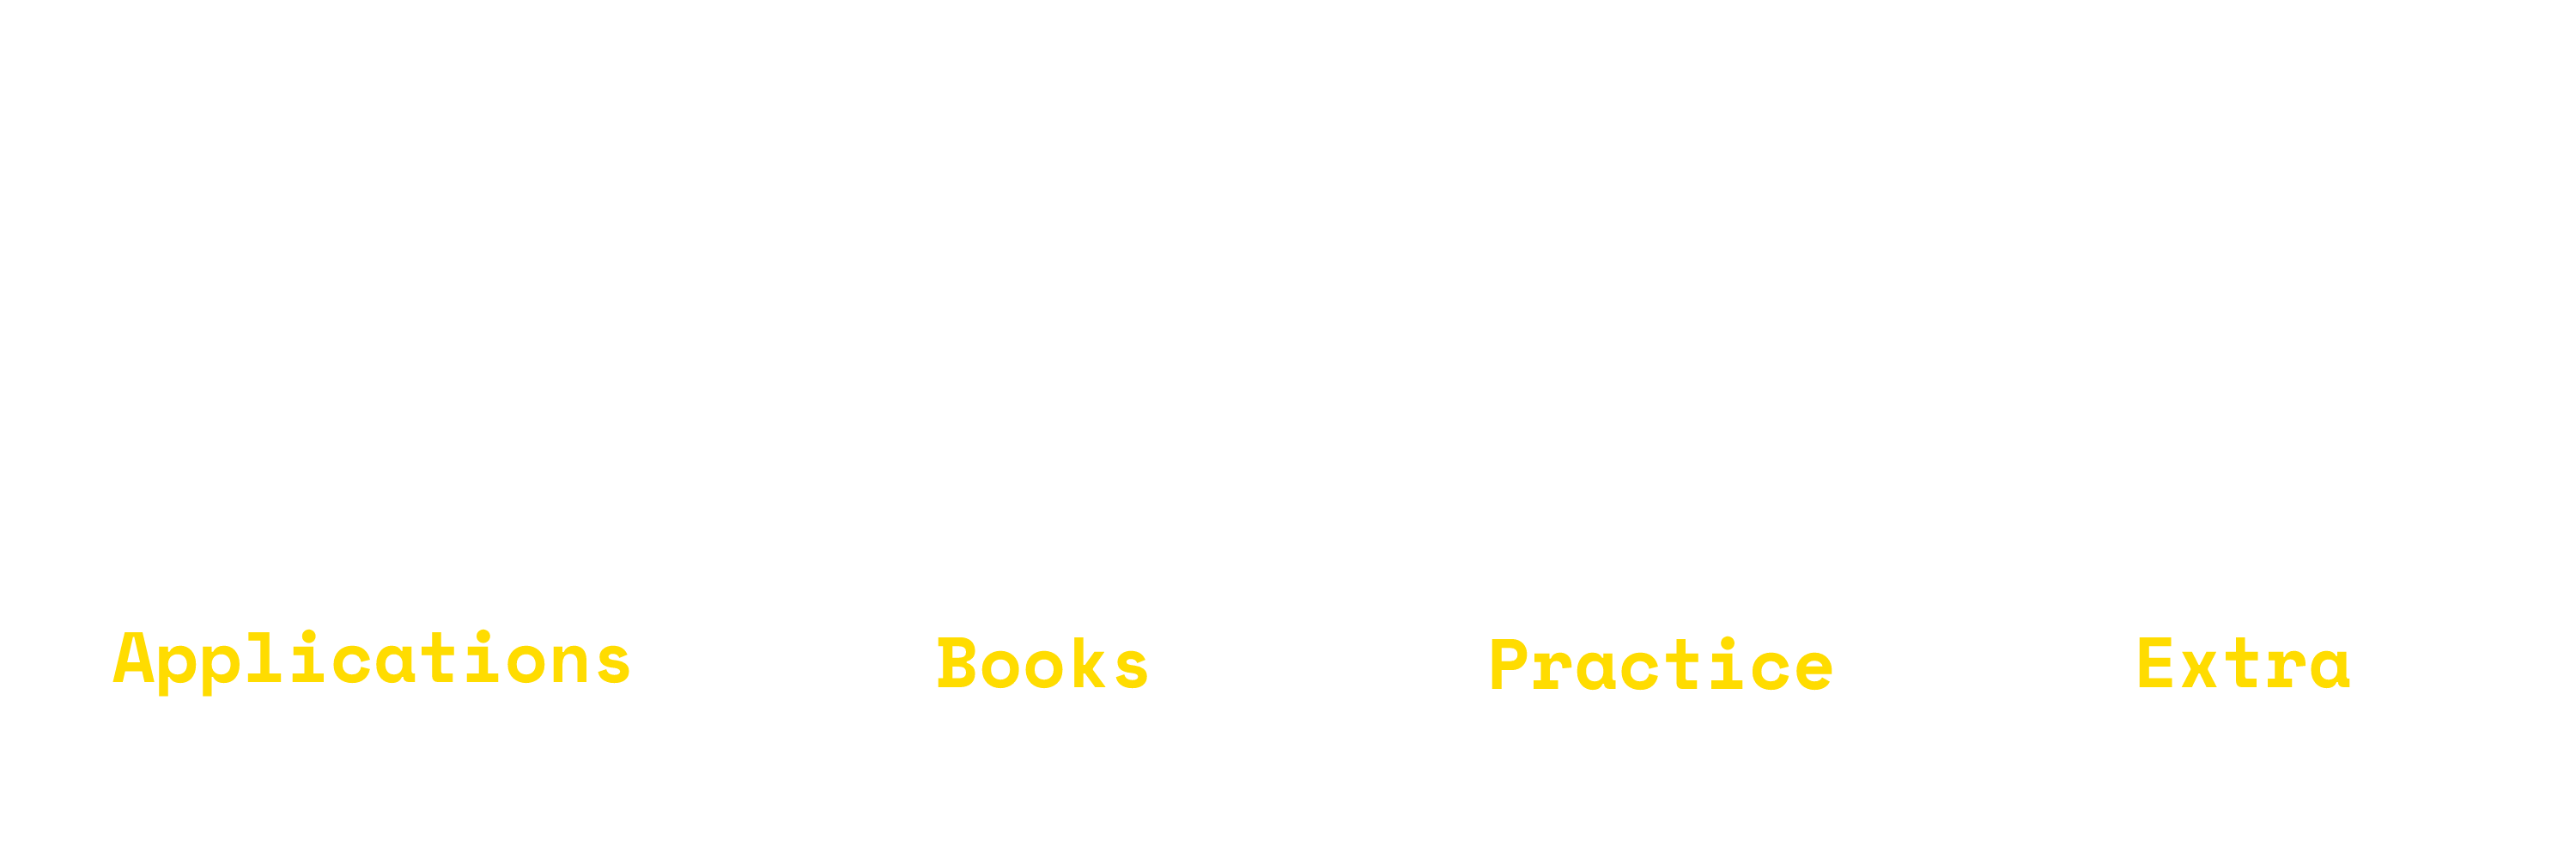
\includegraphics[width=1\linewidth]{graphics/resources.png}
	\end{figure}
	All of these can be found in our repository!\\
	And even more are available online!\\
	\vspace{1cm}
\end{frame}



\framepic{graphics/1.jpg}{
 \textcolor{ucuwhite}{A short history of \\systems programming}
 \vskip 0.5cm
 }

\section{A short history of systems programming}

\begin{frame}{The origins of C}

\begin{wrapfigure}{r}{0.5\textwidth}
\centering
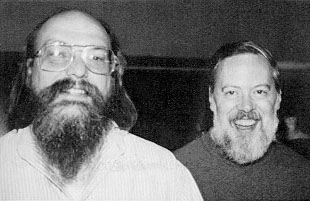
\includegraphics[width=0.5\textwidth]{graphics/ritchie.jpg}
\end{wrapfigure}
\normalsize
The C programming language appeared during Unix development in 1972.\\
\vspace{0.3cm}
Since it was created for a specific purpose % an operating system
and a specific computer, %(PDP-11) 
on the one hand it adapted to the
needs of the programmers, and on the 
other it adopted a large
amount of somewhat unique and unpopular 
ideas and concepts.

\vskip 0.8cm

\end{frame}

\begin{frame}{Possible solutions}
\large
C++ is born to help address some of these problems,\\ 
introduces ‘zero cost’ abstractions, aimed at providing\\
a nice interface for the programmer to use which\\
compiles down to an almost ideal machine code.
\vspace{0.5cm}

Still has the old instruments, hangs on to C's machine\\
model %(the fucking BACKWARDS COMPATIBILITY),
and tries to encourage using the new\\ 
modern safe concepts, 
\href{https://alexgaynor.net/2019/apr/21/modern-c++-wont-save-us/}
{which are not ideal either}.


\end{frame}

\begin{frame}{Modern ideas}

\large
In the meantime, languages like Java, Ruby and\\
Python start sprawling up, presenting another\\
model of growth - they are garbage-collected\\
and are able to present even more complex\\
abstractions (at the expense of the speed).\\

\vspace{0.5cm}

Go and others try to tackle C's speed and\\
low-levelness, 
\href{https://cowlark.com/2009-11-15-go/}{unsuccessfully}.

\end{frame}

\framepic{graphics/1.jpg}{
 \textcolor{ucuwhite}{Pitfalls of the old ways}
 \vskip 0.5cm
 }

\section{Pitfalls of the old ways}

\begin{frame}{Memory layout} 
\inputminted[fontsize=\large]{c}{code/stack.c}
\end{frame}

\begin{frame}{Memory layout} 

\begin{figure}[ht]
	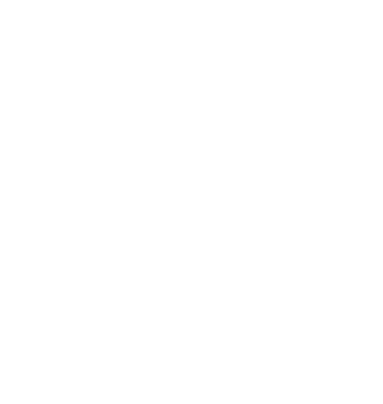
\includegraphics[width=0.4\textwidth]{graphics/stack1.png}
  \hfill
	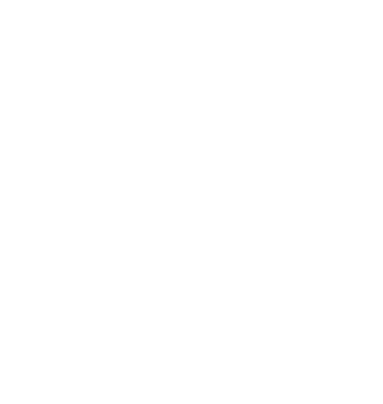
\includegraphics[width=0.4\textwidth]{graphics/stack2.png}
	\hfill
\end{figure}
	
\end{frame}

\begin{frame}{Buffer overflows} 
	\inputminted[fontsize=\large]{c}{code/overflow.c}
\end{frame}

\begin{frame}{Null pointers}
	\inputminted[fontsize=\large]{c}{code/nullp.c}
\end{frame}

\begin{frame}{Dangling pointers} 
	\inputminted[fontsize=\large]{c}{code/danp.c}
\end{frame}

\begin{frame}{Invalidated iterators and double free} 
	\inputminted[fontsize=\large]{c}{code/iter.c}
\end{frame}

\begin{frame}{No real error checking} 
	\inputminted[fontsize=\large]{c}{code/errorcheck.c}
\end{frame}

\begin{frame}{And many more...}
	\Large
	\begin{itemize}[label=$\bullet$]
		\item Memory leak - you can forget to free data
		\item Thread unsafety - another thread can be \\
			modifying the same memory
	\end{itemize}
\end{frame}


\framepic{graphics/1.jpg}{
 \textcolor{ucuwhite}{Where and why is Rust better?}
 \vskip 0.5cm
 }

\section{Where and why is Rust better?}

\begin{frame}{What is Rust?}

\LARGE{\textcolor{ucuyellow}{Safe, Fast, Easy to write. Choose three}}

\vspace{0.8cm}
\large
A modern systems programming language.

\vspace{0.3cm}

First stable version in 2014.\\

\vspace{0.3cm}

Gets rid of unnecessary old ideas, combining \\
them with some of the fresh concepts.
\end{frame}

\begin{frame}{Almost everything makes sense} 

\large
It does not care about C’s old ways\\ 
from the 70s which have been kept up \\
in many languages and systems since.\\ 
%just because (null-char strings, pointers) 

\vspace{0.3cm}
It does not try to needlessly attach new\\ 
stupid things to it. Easily gets rid of bad\\ 
ideas since it’s a young language.\\
\end{frame}

\begin{frame}{Memory safety guarantees}
\large
Rust guarantees, at compile time, that\\
programs are memory-safe.\\

\vspace{0.3cm}

This means:
\begin{itemize}[label=$\bullet$]
	\item No buffer overflows
	\item Everything is bounds-checked if it needs to be
	\item No data races (general thread-safety)
	\item No memory is ever written to by two things at a time
	\item No memory is ever written and read at the same time
\end{itemize}
\end{frame}

\begin{frame}{Tradeoffs}
\large
These guarantees don't\\
come without a cost.

\vspace{0.3cm}

Some of them include:
\begin{itemize}[label=$\bullet$]
	\item Relatively long compile time
	\item You sometimes have to fight with the compiler\\
		(It's always right though, and even tries to help)
	\item A whole new different approach to things
	\item It's a young language!\\
		(This also means you can help)
\end{itemize}
\end{frame}

\begin{frame}{Improvements in almost every field} 
	\large
Rust does not only get rid of the problems\\
of C and garbage-collected languages.
\vspace{0.3cm}

It tries to be better at a lot of other things:
\begin{itemize}[label=$\bullet$]
	\item Super great error handling!
	\item Algebraic data types!\\
		(Functional programming concept)
	\item Advanced macro processing!
	\item Speed increase from C since programs \\
		often know what to expect!
\end{itemize}
\end{frame}

\begin{frame}{An amazing ecosystem} 
%Modern languages are not only language\\
%specifications. Their use almost always\\
%depends on compilers, package management\\
%systems, documentation, formatters, and\\
%test suites!
\vspace{0.25cm}

\large
Rust has a great ecosystem:
\begin{itemize}[label=$\bullet$]
	\item \textcolor{ucuyellow}{rustc} compiler is super helpful, and has great IDE integrations!
	\item \textcolor{ucuyellow}{cargo} is a unified standard for:
		\begin{itemize}[label=$\bullet$]
			\item Package management (pip, yay)
			\item Dependency resolving (setup.py, requirements.txt)
			\item Project management (makefile, CMake)
			\item Testing (gtest etc.)
			\item Documentation (pandoc, asciidoc etc.)
		\end{itemize}
	\item \textcolor{ucuyellow}{rustfmt} is a standard formatter
	\item \textcolor{ucuyellow}{clippy} is a standard linter
\end{itemize}
\vspace{0.55cm}
\end{frame}

\framepic{graphics/1.jpg}{
 \textcolor{ucuwhite}{Basic syntax and ecosystem}
 \vskip 0.5cm
 }

\section{Basic syntax and ecosystem}

\begin{frame}{Hello world!}
	\large
	\textcolor{ucuyellow}{
	All of the code snippets for this lecture\\
	are available in the repository!}
	\vspace{0.5cm}
	\inputminted[fontsize=\Large]{rust}{code/helloworld.rs}
	\vspace{0.4cm}
	\inputminted[fontsize=\Large]{bash}{code/helloworld.sh}

\end{frame}

\begin{frame}{Hello cargo!}
	\inputminted[fontsize=\Large]{bash}{code/hellocargo.sh}
\end{frame}

\framepic{graphics/1.jpg}{
	\textcolor{ucuwhite}{Ownership and lifetimes}
 \vskip 0.5cm
 }

\section{Ownership and lifetimes}
\begin{frame}{Ownership and lifetimes}
	\framesubtitle{Abstract}
	\large
	How would a safe system look like?\\
	\vspace{0.4cm}
	Let's go over a few main points:\\
	\vspace{0.4cm}
	\begin{itemize}[label=$\bullet$]
		\item There can be many readers with no writers at the same time
		\item There can be only one writer with no readers at the same time
		\item Values can be used only as long as they still exist
	\end{itemize}
\end{frame}

\begin{frame}{Ownership and lifetimes}
	\framesubtitle{General}
	\large
	In Rust's terminology, there are two notions of borrowing:
	\begin{itemize}[label=$\bullet$]
		\item Shared reference \textcolor{ucuyellow}{\&}
		\item Mutable reference \textcolor{ucuyellow}{\&mut}
	\end{itemize}

	\vspace{0.5cm}
	Rust forces us to abide by the following principles:
	\begin{itemize}[label=$\bullet$]
		\item Every value has a single owner at any given time.\\
			(You can move a value from one owner to another, but when\\
			value's owner goes away, the value goes away with it too)
		\item You can borrow a reference to a value, for as long as\\
			the reference doesn't outlive the value.\\
			(Borrowed references are temporary pointers, they\\
			allow you to operate with values you don't own)
		\item You can only modify a value when you have exclusive\\
			access to it.
	\end{itemize}
	\vspace{0.5cm}
\end{frame}

\begin{frame}{Ownership and lifetimes}
	\framesubtitle{General}
	\large
	The lifetime of a value starts when it’s created\\
	and ends the last time it’s used.\\
	\vspace{0.2cm}
	Rust computes lifetimes at compile time, we don't\\
	have to do any allocations and frees, Rust borrows\\
	and drops memory for us.
\end{frame}

\begin{frame}{Ownership and lifetimes}
	\framesubtitle{Examples}
	Let's see how Rust automatically drops any values after\\
	their scope ends (and their owner dies):
	\vspace{0.3cm}
	\inputminted[fontsize=\large]{rust}{code/own1.rs}
	\vspace{0.3cm}
	Rust handles all data this way, no matter the complexity,\\
	it will clean up file handlers, network sockets, vectors etc.
\end{frame}

\begin{frame}{Ownership and lifetimes}
	\framesubtitle{Examples}
	\large
	Let's see how Rust handles \textcolor{ucuyellow}{String}s. Does this compile?
	\vspace{0.6cm}
	\inputminted[fontsize=\large]{rust}{code/own2.rs}
\end{frame}

\begin{frame}{Ownership and lifetimes}
	\framesubtitle{Examples}
	\large
	Does this one compile?
	\vspace{0.6cm}
	\inputminted[fontsize=\large]{rust}{code/own3.rs}
\end{frame}

\begin{frame}{Ownership and lifetimes}
	\framesubtitle{Examples}
	\large
	What is different for \textcolor{ucuyellow}{u32}?
	\vspace{0.6cm}
	\inputminted[fontsize=\large]{rust}{code/own4.rs}
\end{frame}

\begin{frame}{Ownership and lifetimes}
	\framesubtitle{Copy and Move}
	\large
	Rust has a special notion which helps it figure\\
	out whether the value should be copied or moved.\\
	\vspace{0.5cm}
	We'll discuss this a bit later, but for now you	can\\
	just remember that Rust copies stack-allocated\\
	primitive values, and moves ownership of heap-\\
	allocated values.
	
\end{frame}

\begin{frame}{Ownership and lifetimes}
	\framesubtitle{Examples}
	\inputminted[fontsize=\large]{rust}{code/own5.rs}
\end{frame}

\begin{frame}{Ownership and lifetimes}
	\framesubtitle{Examples}
	\inputminted[fontsize=\large]{rust}{code/own6.rs}
\end{frame}

\begin{frame}{Ownership and lifetimes}
	\framesubtitle{Examples}
	Let's see how Rust will handle complex correct code:
	\vspace{0.1cm}
	\inputminted[fontsize=\normalsize]{rust}{code/own7.rs}
	\vspace{0.5cm}
\end{frame}

\begin{frame}{Ownership and lifetimes}
	\framesubtitle{Examples}
	\large
	Let's try to invalidate an iterator:
	\vspace{0.3cm}
	\inputminted[fontsize=\large]{rust}{code/own8.rs}
	\vspace{0.5cm}
\end{frame}

\begin{frame}{Ownership and lifetimes}
	\framesubtitle{Examples}
	\large
	Let's try to return a dangling pointer:
	\vspace{0.3cm}
	\inputminted[fontsize=\large]{rust}{code/own9.rs}
	\vspace{0.5cm}
\end{frame}

\begin{frame}{Ownership and lifetimes}
\large	
We've only looked at some of the simplest cases,\\
Rust's system is a lot more complex. We'll go\\
over lifetimes more in the future.\\
\vspace{0.4cm}
Since the concept of a borrow checker is unique to\\
Rust, you will often encounter compiler errors\\
when working until you get used to it.\\
\vspace{0.4cm}
The compiler becomes better and better at working\\
with lifetimes, and provides super helpful errors,\\
but it still can be stressful to fight with it sometimes.
\end{frame}

\framepic{graphics/1.jpg}{
	{Practice - a guessing game}
 \vskip 0.5cm
 }
\section{A simple practice project}

\begin{frame}{Guessing game}
	\framesubtitle{Basics}
	\inputminted[fontsize=\footnotesize]{rust}{code/guess1.rs}
	\vspace{0.4cm}
\end{frame}

\begin{frame}{Guessing game}
	\framesubtitle{Cargo dependencies}
	\Large
	Let's add a random number generator. We have\\
	to add a dependency for \textcolor{ucuyellow}{rand} crate for this.\\
	(crates are Rust's libraries and modules)
	\vspace{0.5cm}

	Add this to your Cargo.toml file:
	\vspace{0.4cm}
	\inputminted[fontsize=\Large]{toml}{code/toml1.toml}
\end{frame}

\begin{frame}{Guessing game}
	\framesubtitle{Random number generation}
	\inputminted[fontsize=\footnotesize]{rust}{code/guess2.rs}
\end{frame}

\begin{frame}{Guessing game}
	\framesubtitle{(Wrong) Input comparison}
	%Match expression, enumerators explanation.*
	\inputminted[fontsize=\normalsize]{rust}{code/guess3.rs}
\end{frame}

\begin{frame}{Guessing game}
	\framesubtitle{Input comparison}
	%Ownership explanation, maybe add a slide about that?*
	\inputminted[fontsize=\normalsize]{rust}{code/guess4.rs}
\end{frame}


\begin{frame}{Guessing game}
	\framesubtitle{Looping}
	\inputminted[fontsize=\normalsize]{rust}{code/guess5.rs}
\end{frame}

\begin{frame}{Guessing game}
	\framesubtitle{Breaking out of the loop}
	\inputminted[fontsize=\large]{rust}{code/guess6.rs}
\end{frame}

\begin{frame}{Guessing game}
	\framesubtitle{Handling invalid input}
	\inputminted[fontsize=\normalsize]{rust}{code/guess7.rs}
\end{frame}

\begin{frame}{More on cargo}
	\inputminted[fontsize=\large]{shell}{code/cargo.sh}
	\vspace{0.5cm}
\end{frame}


\begin{frame}{Interesting readings} 

C, C++ critique:\\

\href{https://web.archive.org/web/19980425023657/http://paul.merton.ox.ac.uk/computing/unix.html}
{Creators Admit UNIX, C Hoax}

\href{https://web.archive.org/web/19990302094922/http://www.elj.com/cppcv3/}
{C++?? : A Critique of C++ (or Programming and Language Trends of the 1990s)}

\href{https://da-data.blogspot.com/2020/10/no-c-still-isnt-cutting-it.html}
{No, C++ still isn't cutting it.}

\vspace{0.5cm}
Rust history:\\ 

\href{https://youtu.be/HiWkMFE8uRE}{C++ \&\& Rust : "Access All Arenas"}

\vspace{0.5cm}
Considering Rust:\\

\href{https://web.archive.org/web/20030625015044/http://www.cs.rice.edu/CS/PLT/Teaching/Talks/TCEA-State-1998/C++/}
{Mastering the AP CS Curriculum Without Using C++}

\href{https://matklad.github.io/2020/09/20/why-not-rust.html}
{Why not Rust?}

\href{https://matklad.github.io/2020/02/14/why-rust-is-loved.html}
{Why is Rust the Most Loved Programming Language?}

\href{http://dtrace.org/blogs/bmc/2018/09/18/falling-in-love-with-rust/}
{Falling in love with Rust}

\href{http://dtrace.org/blogs/bmc/2020/10/11/rust-after-the-honeymoon/}
{Rust after the honeymoon}

\href{http://dtrace.org/blogs/bmc/2018/09/28/the-relative-performance-of-c-and-rust/}
{The relative performance of C and Rust}

\end{frame}

\framepic{graphics/1.jpg}{
	\textcolor{ucuwhite}{Thank you!}
 \vskip 0.5cm
 }

\end{document}
